\clearpage
\section{Automatic Differentiation} \label{sec:ad}
    Tracing is useful in many applications, one of which is Automatic Differentiation (AD).
    Recall how in AD we wish to calculate the derivative of a computer program.
    To do this (in reverse-mode) we wish to calculate the adjoints for the inputs.
    However, to calculate these adjoints, we would first need to calculate the adjoints for the individual computational steps in the program that contribute to an input's sensitivity.
    Of course, it are these steps that are represented in the trace of a program.
    In fact, there is a really close relation between the tapes discussed in Section \ref{sec:bg_ad} and tracing.

    The main difference between the tape used for AD and a regular trace as laid out in Section \ref{sec:tracing}, is the lack of intermediate values in the latter.
    However, provided a trace, we could simply calculate these intermediate values.
    Even better is just storing the intermediate values while we trace a program, this is not really any extra work because these intermediate values are calculated by the tracing function already.
    Consider our trace definition in Listing \ref{lst:traced} as a list of tuples consisting of strings as identifiers and a data constructor denoting the action taken.
    We could just add intermediate values to this structure, but we will soon find this not to be quite enough.
    
    For instance, look at the computational graph in Figure \ref{fig:forward_graph} for $f(x_1,x_2)\coloneqq x_1+(x_1\times x_2)$.
    \begin{figure}[htb]
        \centering
        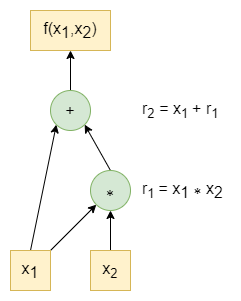
\includegraphics[scale=0.5]{diagrams/forward_example.png}
        \caption{Computational graph of $f(x_1,x_2)\coloneqq x_1+(x_1\times x_2)$}
        \label{fig:forward_graph}
    \end{figure}
    Now, let us say $x_1=5$, and $x_2=3$, and trace it using the method from Section \ref{sec:tracing}.
    This gives us the trace as \texttt{trace\_result} in Listing \ref{lst:forward_trace}.
    This trace is very straightforward: $x_1$ and $x_2$ are assigned their values, and the multiplication is used in the addition, so it shows up first.
    \begin{haskell}[caption=DSL definition of $f$ and its trace, label=lst:forward_trace, gobble=8]
        f :: Value -> Value -> Expression
        f x1 x2 = ELet "x1" (ELift x1) (
            ELet "x2" (ELift x2) (
                EOp2 Add (ERef "x1") (
                    EOp2 Mul (ERef "x1") (ERef "x2")
                )
            ))

        trace_result :: (TValue, Trace)
        trace_result = (TReal "r2" 20.0, [
            ("x1", TLift (TReal "x1" 5.0)),
            ("x2", TLift (TReal "x2" 3.0)),
            ("r1", TOp2 Mul "x1" "x2"),
            ("r2", TOp2 Add "x1" "r1")
        ])
    \end{haskell}
    Now, let us look at the partial derivatives of $f$ in Equation \ref{eq:reverse_ex}, as we would calculate them using chain rule.
    In Equation \ref{eq:reverse_ex2} we see which calculations we need to perform, we define the partial derivatives or ``adjoints'' of a variable $r_i$ as $\bar{r_i}$.
    We also assume here that the ``seed'' value (the value of $\bar{f}$) is one.
    \begin{equation} \label{eq:reverse_ex}
        \begin{aligned}
            \frac{df}{d\vec{x}}=\nabla f&=\begin{bmatrix}
                \frac{\partial r_2(x_1,r_1)}{\partial x_1}\\
                \frac{\partial r_2(x_1,r_1)}{\partial x_2}
            \end{bmatrix}\tran\\
            &=\begin{bmatrix}
                1+\frac{\partial r_2(x_1,r_1)}{\partial r_1}\cdot\frac{\partial r_1(x_1,x_2)}{\partial x_1}\\
                0+\frac{\partial r_2(x_1,r_1)}{\partial r_1}\cdot\frac{\partial r_1(x_1,x_2)}{\partial x_2}
            \end{bmatrix}\tran\\
            &=\begin{bmatrix}
                1+\partial x_1\cdot x_2\\
                \partial x_2\cdot x_1
            \end{bmatrix}\tran
        \end{aligned}
    \end{equation}
    \begin{equation} \label{eq:reverse_ex2}
        \begin{aligned}
            \bar{f}=\bar{r_2}&=1\\
            \bar{r_1}&=\bar{r_2}\times1\\
            \bar{x_2}&=\bar{r_1}\times x_1\\
            \bar{x_1}&=\bar{r_2}\times1\\
            &+\bar{r_1}\times x_2
        \end{aligned}
    \end{equation}
    With our trace and derivative operations defined, we can now look at how we would get from one to the other.
    It is important to start at the output of the program, and since the trace function we defined in Section \ref{sec:tracing} provides us with the named output, we know where to start on our reverse pass.
    In this case, that would be $r_2$.
    As the final value in the primal calculation is the output of the program, its adjoint will be equal to the adjoint of the program or the seed value.
    This is why Equation \ref{eq:reverse_ex2} posits $\bar{f}=\bar{r_2}$.

    Since we are currently working in reverse execution order, we can just use $\bar{r_2}$ to calculate $\bar{x_1}$ and $\bar{r_1}$ directly.
    It should be reiterated that the trace does not encode any explicit information on the order of operations taken while tracing.
    It is of course a list that was built up one operation at the time, but relying on this forces us to do our reverse pass linearly through the trace, which would prevent some task parallelism opportunities.
    Furthermore, while we can also deduce some order from the naming of the intermediate steps (e.g. $r_1$ was done before $r_2$), we should not do this programmatically, because we wish to reserve parallelism opportunities, but also because some intermediate steps might be hidden in the sub-trace of a map.
    Luckily, we can also discover the ``ancestors'' of any step in the trace by looking at the traced operation.
    For $r_2$ the traced operation was \texttt{TOp2 Add "x1" "r1"}, so we know that for our reverse pass, we next want to look at $x_1$ and $r_1$, as their adjoints (or part of them) rely on the value of $\bar{r_2}$ (which we can also see in Equation \ref{eq:reverse_ex2}).
    For now we will gloss over how we decide which ancestor adjoint to compute first, and just look at the adjoint of $r_1$.
    
    We know that $\bar{r_1}$ is dependent on $\bar{r_2}$, but how exactly is defined by the operation that produced $r_2$, which in this case is addition.
    Now, addition is really simple, as the derivative of addition of two values is the addition of the derivatives of those values.
    See Equation \ref{eq:reverse_add}, where we calculate the adjoint $\bar{r_1}$ and see how this addition just resolves to one.
    \begin{equation} \label{eq:reverse_add}
        \begin{aligned}
            \bar{r_1}&=\bar{r_2}\cdot\frac{\partial r_2}{\partial r_1}\\
            &=\bar{r_2}\cdot\frac{\partial(x_1+r_1)}{\partial r_1}\\
            &=\bar{r_2}\cdot1
        \end{aligned}
    \end{equation}

    We can again find the ancestors of $r_1$ by looking at the trace, where we find $x_1$ and $x_2$.
    Let us look at $x_2$ first.
    $\bar{x_2}$ is dependent on $\bar{r_1}$, which we just calculated, but rather than an addition (like $r_2$), $r_1$ is a multiplication.
    We mentioned in Section \ref{sec:bg_ad}, in Equation \ref{eq:dualnumbers}, how the derivative of a multiplication uses both the primal part and the derivative part of a number.
    To get $\bar{x_2}$ we realize (as is visible in Equation \ref{eq:reverse_ex2} as well), that we need the primal value of $x_1$.
    We mentioned before we needed the intermediate values, and this is why.
    Multiplication is not the only operation that requires a primal component, but it is a prime example.
    We see in Equation \ref{eq:reverse_mul} how this adjoint resolves to use the primal component $x_1$.
    \begin{equation} \label{eq:reverse_mul}
        \begin{aligned}
            \bar{x_2}&=\bar{r_1}\cdot\frac{\partial r_1}{\partial x_2}\\
            &=\bar{r_1}\cdot\frac{\partial(x_1x_2)}{\partial x_2}\\
            &=\bar{r_1}\cdot x_1
        \end{aligned}
    \end{equation}

    Now would also be a good time to quickly reflect on the difference between the tangent (from forward-mode AD) and the adjoint.
    In forward-mode AD, the operation taken to produce some variable, would influence the tangent of that variable.
    This is somewhat intuitive, $r_1$ is a multiplication, and its tangent is $\dot{r_1}=\dot{x_1}\times x_2+\dot{x_2}\times x_1$.
    However, this is not the case for reverse-mode AD.
    In reverse-mode, we see that this information gets passed on to the adjoints of the variable used by the operation, rather than the variable it produced.
    It should be clear why: the tangents denote how the variable is influenced by a change in the inputs, while an adjoint denotes how its corresponding variable influence the outputs.
    It is important to closely observe this, mainly for implementation purposes: we want to calculate (part of) the adjoint before we actually arrive at that step in the trace.
    To calculate $\bar{x_2}$ we need to know what variable $x_2$ was multiplied with (namely $x_1$).
    This means that if we do not want to helplessly bounce around through our trace looking for references (to $x_2$ for example), it would be better to calculate (the relevant part of) $\bar{x_2}$ while we still see how it is being used.\\
    This then also bring us neatly to our next conundrum: what if a variable is used multiple times.
    In the example, this goes for $x_1$, something that we have ignored until now.
    The mathematical solution is simple: the partial derivative of a variable that is used multiple times, is just a summation of the adjoints arising from those uses.
    We see this in Equation \ref{eq:reverse_ex2}, where $\bar{x_1}$ is calculated by adding the influence from $r_1$ and the influence from $r_2$ together.
    However, implementation-wise this can be a bit of a hurdle.

    As mentioned, the trace is not in any order.
    This is unlike a typical Wengert list or tape.
    While assuring some order beforehand, or doing topological sort on the computational graph described by the trace, will in large part solve this problem, it also enforces linear execution of the reverse pass.
    And while it is not something we will linger on for now, allowing for concurrency or task parallelism while calculating the derivative, might be a nice for a performance boost, and complement the inherit data-parallelism opportunities of array operations.
    So, to solve this, we want to include some form of reference counting.
    During the forward-pass we could count how many times each variable is used in the trace, since we need to store intermediate values anyways, keeping a counter for each of these variables seems like little extra work.
    Now, on the reverse pass we can check these reference counters and every time we find part of the adjoint for a variable, we decrement its associated counter.
    If a counter has not reached zero after we have decremented it, we know its adjoint is not yet complete, and we can ignore it for now.
    If it has we can add up all the parts of the adjoint and continue from there.
    Provided there is only one output to the program, we know that all reference counters will eventually reach zero, and therefor we are assured we will calculate all adjoints.
    However, this provision is not as clear cut as it seems.
    Currently our DSL does not really have any room for multiple outputs, and as it is functional does not support any side-effects.
    Instead, to provide multiple outputs, currently the only way is to output an array.
    If we keep arrays in the trace, an array as output would still count as a single value.
    There is a slight discrepancy between the trace and the output if we trace away arrays however: the program will still output an array, but only its individual items are able to be found in the trace.
    This is not really a big problem, since the name of these individual outputs are derived from the name of the full array, but also because it would make little sense to trace away arrays from a program that outputs an array.

    So, we find that our trace needs to be extended with two additional things in the forward pass: intermediate values and reference counters.
    We do this in Listing \ref{lst:forward}, in the data type \texttt{Forward}.
    We also introduce a clone of the \texttt{Traced} data type as \texttt{Forwarded}, as we need to reference the new \texttt{Forward} type in the constructors for maps and vectorized maps.
    We also replace the list structure of \texttt{Trace} with a key-value map.
    This is not strictly necessary, but it allows us to more quickly access the values in the map, while also clearly communicating there is no pre-set order to the trace.
    Each value in a \texttt{Forward} map is a 3-tuple consisting of respectively: the intermediate value, the traced operation performed, and the reference counter for this variable.
    Other than the added reference counting, and saving of intermediate values, the tracing process remains the same as it was in Section \ref{sec:tracing}.

    \begin{haskell}[caption=Forward pass data structures, label=lst:forward, gobble=8]
        data Forwarded
            = FLift TValue
            | FOp0  Op0
            | FOp1  Op1       String
            | FOp2  Op2       String String
            | FMap  [Forward] String
            | FMapV Forward   String

        type Forward = Map String (TValue, Forwarded, Int)
    \end{haskell}

    \subsection{The Reverse Pass}
        As discussed, to facilitate our reverse pass we need both the reference counting and intermediate values.
        Now let us define a function \texttt{reverse} that does the reverse pass.
        This reverse pass should find all the adjoints in the program.
        So, it should take in an object of the \texttt{Forward} type and output a map containing the adjoints.
        In Listing \ref{lst:reverse_def} we define constructors for adjoints: one for arrays, one for sparse arrays (represented by a single index and the associated value), one for real values, and a ``null'' value we can use as a placeholder.
        We also define the \texttt{Reverse} type, which will contain these adjoints, and which is returned at the end of the reverse pass.
        The \texttt{Reverse} type maps the names of each part of the calculation to a 2-tuple containing a list of contributions of other adjoints, and its own final adjoint.

        \begin{haskell}[caption=Definition of the \texttt{Reverse} type, label=lst:reverse_def, gobble=12]
            data Adjoint
                = AArray  [Float]
                | ANull
                | AReal   Float
                | ASparse Int Float

            type Reverse = Map String ([Adjoint], Adjoint)
        \end{haskell}

        With our data types defined, we can now look at the first cases of reverse AD.
        In Listing \ref{lst:reverse} we define two functions: \texttt{reverse'} which will do most of the actual reverse pass, and a wrapper function called \texttt{reverse}.
        To assign the adjoints in the \texttt{Reverse} map, we define a function \texttt{seedAncestors}.
        This function, given in Listing \ref{lst:seedanc}, for a specified item in the trace, finds and adds the adjoints to the ancestors of this item (the ancestors in the computational graph).
        To do this it needs to transform and combine adjoints of differing dimensions, to do this it uses the utility functions \texttt{toSingle}, \texttt{toArray}, \texttt{sumAdjoints}, and \texttt{combineAdjoints}.
        These functions are defined in Listing \ref{lst:combine}, which we will discuss in a bit.
        It also uses a utility function \texttt{getAncestors} which simply finds the ancestors of a trace item by looking at the specific step made; it is defined in Appendix \ref{app:utility}.
        An important thing to note here is that if the \texttt{seedAncestors} function calculates the final adjoint of a node, when it is available.
        This means that \texttt{reverse'} can just look at whether or not the final adjoint of a node is available, and only continue when it is.
        If it is not, we can be assured it will be calculated later, as the path to the output to the node in question should be calculated still. % NOTE: Dit is misschien een beetje vaag
        
        \begin{haskell}[caption={The reverse pass function. \texttt{reverse} takes in a forward-pass trace, the name of the output of the program as a string, and the seed value (the adjoint of the output); and outputs a map containing all adjoints. \texttt{reverse'} takes in a forward-pass trace, a queue of items in the trace that still need to be passed on the reverse pass, and the current map of adjoints; and ouptuts the updated map of adjoints (from resolving the first item in the queue).}, label=lst:reverse, gobble=12]
            reverse :: Forward -> String -> Adjoint -> Reverse
            reverse t s v = reverse' t a r
                where
                    r = seedAncestors t (Map.singleton s ([], v)) s
                    a = getAncestors t s

            reverse' :: Forward -> [String] -> Reverse -> Reverse
            reverse' _ []     r = r
            reverse' t (s:ss) r = case r Map.! s of
                (_, ANull) -> reverse' t ss r
                (_, a)     -> reverse' t ss'' r'
                where
                    (r', ss') = seedAncestors t r s a
                    ss''      = ss ++ ss'
        \end{haskell}

        It is the \texttt{seedAncestors} function that does most of the work.
        The string passed to it is the name of the node whose ancestors need to be seeded.
        This is the node which determines how the adjoints its ancestors' adjoints are transformed.
        We see in Listing \ref{lst:seedanc} how we have different cases for the different constructors in our \texttt{Forwarded} class.
        For variable instantiation and nullary operations the result is simple: since they have no ancestors they do not influence any adjoints.
        
        The unary operations are already more complicated, mostly because both of them are used on arrays.
        The idea behind indexing is very simple: indexing is a lot like variable reference.
        Since nothing happens when indexing, nothing should happen on the reverse pass either, except of course that the adjoint of the new variable is part of the adjoint of the array it was indexed from.
        It should also be noted that indexing as an operation in the forward pass will only be present if we chose to not trace away arrays.
        If we did trace away arrays with our forward pass, indexing operations would really be nothing more than variable reference, which would vanish in the trace.
        This also means that the ancestor of the indexing operation is an array.
        It is now important to realize that for a variable in the program, its adjoint will be of the same type.
        This is not something we really think about with real numbers, however when we want to get the adjoint of an array, it can not be a real number, as the array's items may be used separately of each other and could therefor have different individual adjoints.
        When we bring this back to indexing this seems somewhat obvious as well, it is not the whole array that influenced the variable that, it was only the indexed variable.
        This gives us a clear idea of the derivative for an array that was indexed on: an array with the tangent or adjoint at the index that was indexed, and zeroes for every other item.
        This mimics how we would extract a singleton value from a vector, which is effectively what we are doing, only in the differentiated part of the number.
        In Listing \ref{lst:seedanc} we see this because we add a \texttt{ASparse} adjoint to the ancestor of the indexing operation.
        These reperesent a sparse array where the first argument is the index of the only non-zero item, and the second item is that value.

        For the sum operation our earlier observation about how the adjoint of an array is an array as well comes into play again.
        The sum operation, like indexing, also only applies to arrays, however instead of only using one element of the array, it instead uses all of them.
        What helps here is that we can imagine the sum operation as a regular list of additions.
        The reverse pass over an addition operation is very simple: the adjoint of the variables that are added together are equal to the adjoint of the sum.
        Now when we extend this to our array, we see that the (partial) adjoint of the array that is summed, is just an array with the adjoint of the sum for every item in array.

        \begin{haskell}[caption={Function for seeding ancestors of a node. \texttt{seedAncestors} takes in the forward-pass trace, the current reverse pass map, the name of the item to seed the ancestors of, and the adjoint of that item to seed its ancestors with; and outputs a tuple containing an updated reverse pass, and a list of strings of items to evaluate to add to the reverse pass queue.}, label=lst:seedanc, gobble=12]
            seedAncestors :: Forward -> Reverse -> String -> Adjoint -> (Reverse, [String])
            seedAncestors t r s a = case traced of
                FLift _        -> (r, [])
                FOp0  _        -> (r, [])

                FOp1  op s1    -> case op of
                    Idx i -> (addAdjoint r s1 (ASparse i (toSingle a)), [s1])
                    Sum   -> (addAdjoint r s (AArray (toArray a)), [s1])
                
                FOp2  op s1 s2 -> case op of
                    Add -> 
                        let r1 = addAdjoint r  s1 (AReal (toSingle a))
                            r2 = addAdjoint r1 s2 (AReal (toSingle a))
                        in  (r2, [s1, s2])
                    Mul ->
                        let r1 = addAdjoint r  s1 (AReal ((toSingle a) * intermediateF s2))
                            r2 = addAdjoint r1 s2 (AReal ((toSingle a) * intermediateF s1))
                        in  (r2, [s1, s2])
                    Sub ->
                        let r1 = addAdjoint r  s1 (AReal (toSingle a))
                            r2 = addAdjoint r1 s2 (AReal (-1 * toSingle a))
                        in  (r2, [s1, s2])
                
                FMap  fss s1   ->
                    let (r1, as, ss) = seedMap fss r s 0
                    in  (addAdjoint r1 s1 as, s1 : ss)
                
                where    
                    addAdjoint :: Reverse -> String -> Adjoint -> Reverse
                    addAdjoint z s b =
                        let as' = b : as
                        in  case t Map.! s of
                            (_, f, c) ->
                                if   length as' == c
                                then Map.insert s (as', combineOrSumAdjoints f as') z
                                else Map.insert s (as', ANull) z
                        where
                            as = case Map.lookup s z of
                                Just (v, _) -> v
                                Nothing     -> []

                    traced :: Forwarded
                    (_, traced, _) = t Map.! s

                    intermediateA :: String -> [Float]
                    intermediateA s = case t Map.! s of
                        (TArray _ v, _, _) -> v
                        _                  -> error "Intermediate not an array"

                    intermediateF :: String -> Float
                    intermediateF s = case t Map.! s of
                        (TReal _ v, _, _) -> v
                        _                 -> error "Intermediate not a float"
        \end{haskell}

        Our binary operations are relatively simple, as they are very standard and do not involve arrays.
        We just discussed how addition just ``passes'' its adjoints through to its ancestors, and the same goes for subtraction.
        That just leaves us with multiplication.
        Here we see the first use of our intermediate values.
        Using the \texttt{intermediateF} function, we extract the intermediate values from a multiplication's ancestors from our forward pass.
        We then multiply those by the adjoint, and pass them on the appropriate ancestor.

        \begin{figure}[htb]
            \centering
            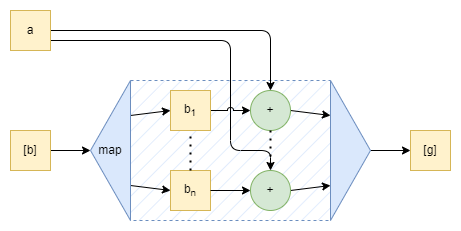
\includegraphics[scale=0.5]{diagrams/map_example.png}
            \caption{Computational graph of $g(a,\vec{b})\coloneqq\texttt{map}\ (+a)\ \vec{b}$}
            \label{fig:map_graph}
        \end{figure}

        Now we come to the map operations, which are more complicated.
        Examine the computational graph in Figure \ref{fig:map_graph}, where we map a simple addition over an array.
        In this figure, the map is displayed as a box, because in our trace maps are stored as separate sub-traces.
        This might seem a little silly for a simple addition, but since maps can take any function (within the bounds of the DSL), we need to account for more complicated functions as well (e.g. including control flow, etc.)
        Furthermore, highlighting the map as a box or context on its own highlights and interesting property: this context may access variables in the wider context.
        We also need to consider the adjoints for these variables in the ``closure'' of the function.
        While it might be tempting to just run our existing reverse pass functions on these sub-traces, we would still need to gather the adjoints into a single adjoint array as the adjoint for the original array.
        Furthermore, it starts to become muddy what to do with variables that are used by the map, but are not contained within it, like $a$ in Figure \ref{fig:map_graph}.
        We also do not want our reverse pass to start leaking out of the map operation: in Figure \ref{fig:map_graph}, this would happen if we accidentally continued our reverse pass for $a$, while that is actually out of scope of our map operation, and should be done by the main reverse pass.
        Which leads us to another problem: what if a variable is only used in the context of a map (again like $a$ in Figure \ref{fig:map_graph}), if we do not follow it up within the reverse pass in the map, we need to add it to the queue of the main reverse pass.
        In Figure \ref{fig:map_graph}, $a$ is an informal ancestor of the map operation, one that is not immediately obvious (especially not in more complex mapped functions).
        
        All this is why, in Listing \ref{lst:rev_maps}, we introduce the \texttt{seedMap} function, that is specifically made for continuing the reverse pass within a map.
        It uses \texttt{seedAncestors} to still calculate and pass the adjoints within our map, but it makes sure only the straight-line function of a single item in the map is explored, any other variables that are used in the map trace are given their adjoints, but not explored: they are instead stored and added to the main reverse pass' queue.
        It might be important to reiterate here that since these traces are single-line programs, and due to the nature of functional programming, only one ancestor of any action is within the context of the sub-trace, while all others should be from the main context.
        Other items in the array that is mapped over are also considered in the main context, since the sub-traces only traces the map over a single item.
        Very important is also that intermediate values in this context cannot escape this context in any ways.
        They can not be used by other parts of the program, as they are all locked away in the map operation.
        (If this were possible, it would violate the functional nature of the program.)

        In Listing \ref{lst:rev_maps} we see this all coming together.
        The \texttt{seedMap} function loops over the sub-traces to get their adjoints (and any outside variables that need visiting).
        Then \texttt{seedMap'} uses \texttt{seedAncestors} to actually move the reverse pass through a single sub-trace, and to get the final adjoint.
        The \texttt{findAncestor} function is used to find which of the found ancestors is actually in the sub-trace, and which ones come from outside the sub-trace's context.

        \begin{haskell}[caption={Functions for the reverse pass through maps. \texttt{seedMap} takes in the array of sub-traces used in the map, the current reverse map, the adjoint of the map's output array, the name of the map's output array, and an integer for keeping track of the index the function is currently on. It returns a 3-tuple containing the updated reverse map, the adjoint of the whole map operation, and a list of names of items that were affected by the map to add to the queue. \texttt{seedMap'} takes in a single sub-trace, the current reverse map, the adjoint of the map's output array, and the name of the map's output array. It also returns the a 3-tuple, with the updated array, the adjoint for this specific sub-trace, and a list of names of affected items in the trace.}, label=lst:rev_maps, gobble=12]
            seedMap :: [Forward] -> Reverse -> Adjoint -> String -> Int
                -> (Reverse, Adjoint, [String])
            seedMap []     r _ _ _ = (r, AArray [], [])
            seedMap (f:fs) r a s c =
                let si                  = s ++ '!' : show c
                    (AArray as)         = a
                    ai                  = AReal (as !! c)
                    (ra, AReal  aa, sa) = seedMap' f r ai si 
                    (rr, AArray ar, sr) = seedMap fs ra s (c + 1)
                in (rr, AArray aa : ar, sa ++ sr)

            seedMap' :: Forward -> Reverse -> Adjoint -> String
                -> (Reverse, Adjoint, [String])
            seedMap' f r a s =
                let (rr, sr) = seedAncestors f r s a
                    (sc, so) = findAncestor sr
                in  case sc of
                    Just sn -> 
                        let (rf, af, sf) = seedMap' f rr (getAdjoint rr sn) sn
                        in  (rf, af, so ++ sf)
                    Nothing -> (rr, a, so)
                where
                    getAdjoint :: Reverse -> String -> Adjoint
                    getAdjoint r s = case Map.lookup s r of
                        Just (_, a) -> a
                        Nothing     -> ANull
                    
                    findAncestor :: [String] -> (Maybe String, [String])
                    findAncestor []     = (Nothing, [])
                    findAncestor (c:cs) =
                        let (cr, crs) = findAncestor cs
                        in  case cr of
                            Just cr' -> if cr' == c then (cr, crs) else (cr, c : crs)
                            Nothing  ->
                                if   Map.member c f 
                                then (Just c, crs)
                                else (Nothing, c : crs)
        \end{haskell}

        For vectorized maps (\texttt{FMapV} in the forward pass) the process is very similar, however we now use the single sub-trace to calculate the adjoints.
        Since the essence of the vectorization means that all items in the array follow the same path, we can calculate the adjoint for each item at the same time using data parallelism.

        We mentioned transforming and combining adjoints briefly before, but it is something we should look into further.
        First off, as mentioned before, adjoints of real numbers need to be real numbers, and adjoints of arrays need to be arrays as well.
        However, some operations in our DSL transform an array into a single number (like sum or indexing), meaning the reverse derivative needs to transform these adjoints from real numbers back into arrays.
        The functions \texttt{toSingle} and \texttt{toArray} in Listing \ref{lst:combine} make these transformations, or assure the adjoints are in the right shape.
        The \texttt{toArray} also takes in an integer that represents the length of the array, as we need the adjoint arrays to be the same size of the primal arrays.
        % TODO: Check if the uses of toArray provide the length of the array

        Furthermore, we also need to sum partial adjoints into a single adjoint.
        This is fairly simple to do for real values, which happens in \texttt{sumAdjoints} in Listing \ref{lst:combine}.
        The arrays are little more in-depth however, since they need to be summed up element-wise.
        This is what happens in \texttt{combineAdjoints}.
        We also define a utility function \texttt{combineOrSumAdjoints} which looks at the current step from the trace to determine whether \texttt{combineAdjoints} or \texttt{sumAdjoints} should be used.
        
        \begin{haskell}[caption={Functions to transform and combine adjoints. \texttt{combineOrSumAdjoints} takes in a step in a trace, and its list of adjoints, and then uses either \texttt{sumAdjoints} or \texttt{combineAdjoints} to return the adjoint for that step. \texttt{combineAdjoints} combines the input adjoints into a single array adjoint. \texttt{sumAdjoints} sums its input adjoints to a single real adjoint. \texttt{toSingle} takes in an adjoint, transforms it into a real adjoint if necessary, and then returns that real as a float. \texttt{toArray} takes in an adjoint and an integer representing length and transforms these into an array adjoint, returning that array adjoint as an array of floats.}, label=lst:combine, gobble=12]
            combineOrSumAdjoints :: Forwarded -> [Adjoint] -> Adjoint
            combineOrSumAdjoints (FOp1  Idx _) = combineAdjoints
            combineOrSumAdjoints (FOp1  Sum _) = combineAdjoints
            combineOrSumAdjoints (FMap  _   _) = combineAdjoints
            combineOrSumAdjoints (FMapV _   _) = combineAdjoints
            combineOrSumAdjoints _             = sumAdjoints

            combineAdjoints :: [Adjoint] -> Adjoint
            combineAdjoints [x]     = x
            combineAdjoints (x:y:z) = combineAdjoints (ca x y : z)
                where
                    ca :: Adjoint -> Adjoint
                    ca (AArray as) (AArray bs)   = AArray (zipWith (+) as bs)
                    ca (AArray as) (ASparse i b) = AArray
                        (take index as ++ [as !! index + b] ++ drop (index + 1) as)
                    ca (ASparse i b) (AArray as) = AArray
                        (take index as ++ [as !! index + b] ++ drop (index + 1) as)
                    ca _           _             = error "Can only sum arrays"
            
            sumAdjoints :: [Adjoint] -> Adjoint
            sumAdjoints [x]     = x
            sumAdjoints (x:y:z) = sumAdjoints (sa x y : z)
                where
                    sa :: Adjoint -> Adjoint -> Adjoint
                    sa (AReal rx) (AReal ry) = AReal (rx + ry)
                    sa _          _          = error "Can only sum singles"
    
            toSingle :: Adjoint -> Float
            toSingle (AArray vs)   = sum vs
            toSingle ANull         = error "Tried to simplify null adjoint"
            toSingle (AReal v)     = v
            toSingle (ASparse _ v) = v
    
            toArray :: Adjoint -> Int -> [Float]
            toArray (AArray v) l =
                if   length v == l
                then v
                else error "Array of wrong length"
            toArray ANull        l = error "Tried to make array from null adjoint"
            toArray (AReal v)    l = repeat l v
                where
                    repeat :: Int -> Float -> [Float]
                    repeat 0 _ = []
                    repeat i v = v : repeat (i - 1) v
            toArray (ASparse i v) l = take i zeroes ++ [v] ++ take (l - i - 1) zeroes
                where
                    zeroes :: [Float]
                    zeroes = 0.0 : zeroes
        \end{haskell}

        With this we have covered all possible statements in our forward-pass trace, meaning we could use the \texttt{reverse} function to find all the adjoints from a given trace.
        The map it returns allows us to look up any adjoint in the trace, most importantly the adjoints of the input variables, which form the gradient of the function.